\section{Cinematica Manipolatore}
L'obiettivo di questa sezione è quello di andare ad illustrare le metodologie che hanno permesso di ottenere sia la cinematica diretta che quella inversa, entrambe per posizione, velocità ed accelerazione.
\par Prima di proseguire nei paragrafi seguenti è necessario definire una tabella con i principali parametri del robot:
\begin{table}[h!]
\centering
\begin{tabular}{|c |c |c|} 
 \hline
 Nome & Descrizione  & Valore \\ [0.5ex] 
 \hline\hline
 $l [m]$ & lunghezza link  & 0.25 \\ 
 $m [kg]$ & massa link & 2.9 \\
 $c_m [m]$ & posizione centro di massa & 1.25 \\
 $J_r [kg\cdot m^2]$ & momento d'inerzia baricentrico & $5.22\cdot 10^{-2}$ \\
 $d [m]$ & lunghezza semitelaio & 0.09 \\
 \hline
\end{tabular}
\caption{Parametri manipolatore}
\label{table:1}
\end{table}
\\Tutti e quattro i link hanno lunghezza, massa, posizione del centro di massa e momento di inerzia uguali, per questo si è deciso di rappresentare i dati una sola volta.
\begin{figure}[ht]
\begin{center}
    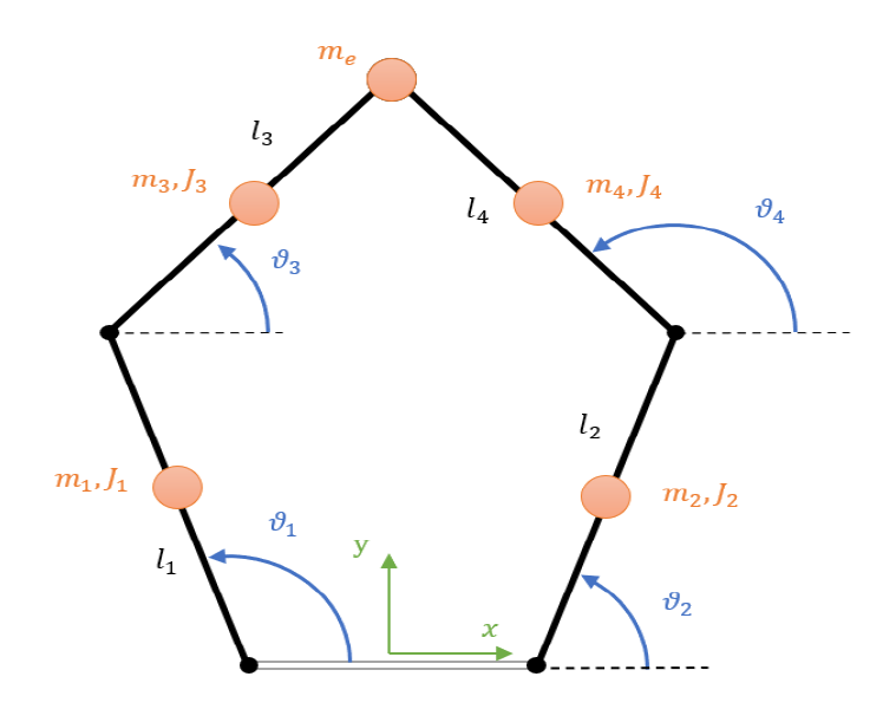
\includegraphics[scale=0.6]{Immagini/Robot2.png}
    \caption{Rappresentazione fisica del robot \label{fig:Robot1}}
\end{center}
\end{figure}
\subsection{Cinematica Diretta}
La cinematica diretta si occupa di trovare il legame tra i parametri interni del robot e la posa che esso assume, per posa si intende la posizione e l'orientamento. In questa sezione vi sarà un'analisi sulla cinematica diretta di posizione, velocità ed accelerazione.
\subsubsection{Posizione}\label{sec:Cinematica-pos}
Nella cinematica diretta di posizione, a partire dal robot e da $\theta_1$ e $\theta_2$, si riesce a ricavare la posizione dei link non motorizzati, i loro angoli, che sono rispettivamente $\theta_3$ e $\theta_4$ e la posizione $[x,y]$ dell'\textit{end-effector}.
L'approccio utilizzato per il calcolo della cinematica diretta è stato quello delle equazioni alle circonferenze, in particolare vengono definite due equazioni:
\begin{itemize}
	\item Circonferenza centrata in E1 che passa per l'end-effector e la base del primo link
	\item Ciconferenza centrata in E2 che passa per l'end-effector e la base del secondo link
\end{itemize}
\begin{figure}[ht]
	\begin{center}
		\includegraphics[scale=0.65]{Immagini/EqCirc}
		\caption{Equazioni alle circonferenze \label{fig:eqCirc}}
	\end{center}
\end{figure}
Dalla combinazione di queste due si ottiene il seguente sistema:
\begin{equation}
    \begin{cases}
    (x-\frac{l}{2}-l\cos\theta_1)^2+(y-l\sin\theta_1)^2 = l^2 \\
    (x+\frac{l}{2}-l\cos\theta_2)^2+(y-l\sin\theta_2)^2 = l^2
    \end{cases}
\label{eq:CinCirc}
\end{equation}
Da queste, andando a sviluppare i calcoli si ottiene:
\begin{equation}
	\begin{cases}
		x^2+x(-2d-2l\cos\theta_2) +y^2+y(-2d\sin\theta_2) + d(d+2l\cos\theta_2) = 0 \\
		x^2+x(2d-2l\cos\theta_1) +y^2+y(-2d\sin\theta_1) + d(d-2l\cos\theta_1) = 0
	\end{cases}
\label{eq:CinCirc2}
\end{equation}
Andando a sottrarre le equazioni:
\begin{equation*}
	x(-4d-2l(\cos\theta_2-\cos\theta_1)) + y(-2l(\sin\theta_2-\sin\theta_1))+2ld(\cos\theta_2+\cos\theta_1) = 0
\end{equation*}
Una volta risolto è possibile ricavare x in funzione di y come:
\begin{equation}
	x = \frac{y\cdot l(\sin\theta_2 - \sin\theta_1)-l\cdot d(\cos\theta_2+\cos\theta_1)}{-2d-l(\cos\theta_2-\cos\theta_1)}
\end{equation}
Sostituendo la x nelll'eqazione \ref{eq:CinCirc} è possibile ricavare y come: 
\begin{equation*}
	y_{1,2}\footnote{$\Delta = \sqrt{B^2-4AC}$} = \frac{-B \pm \Delta}{2A} 
\end{equation*}
Dove i parametri A,B e C sono:
\begin{equation*}
    A = l^2 (\sin\theta_2- \sin\theta_1)^2 + (-2 d-l (\cos\theta_2 - \cos\theta_1))^2
\end{equation*}
\begin{equation*}
\begin{aligned}
   B =  -2 l^2 d (\sin\theta_2-\sin\theta_1)  (\cos(\theta_2+\theta_1) + l(\sin\theta_2-\sin\theta_1)   (-2d-l(\cos\theta_2-\cos\theta_1))\\ (-2d-2l\cos\theta_2) - 2l\sin\theta_2 (-2d-l(\cos\theta_2-\cos\theta_1))^2
\end{aligned}
\end{equation*}
\begin{equation*}
\begin{aligned}
    C = l^2 d^2 (\cos\theta_2+\cos\theta_1)^2-l d (\cos\theta_2+\cos\theta_1)(-2d-l(\cos\theta_2-\cos\theta_1) ) \\ (-2d-2l\cos\theta_2)+(d^2+2dl\cos\theta_2)(-2dl(\cos\theta_2-\cos\theta_1))^2
\end{aligned}
\end{equation*}
Il passo successivo è quello di ricavare la posizione $P=[x,y]$ dell'end-effector. La formula della y fornisce due risultati diversi, in una caso quando si utilizza $+\Delta$ e l'altro quando si usa $-\Delta$. Per come è modellato il manipolatore, l'unica soluzione fisicamente raggiungibile è quella con delta positivo. 
Il passo successivo è quello di andare a trovare le posizioni dei giunti non motorizzati mediante relazioni geometriche nel seguente modo: 
\begin{equation*}
    E_{1X} = -d+l\cdot \cos\theta_1 \ \ \  E_{1Y}=l\cdot \sin\theta_1
\end{equation*}
e
\begin{equation*}
    E_{2X} = d+ l\cdot \cos\theta_2 \ \ \  E_{2Y} = l\cdot \sin\theta_2
\end{equation*}
Si possono trovare gli angoli $\theta_3 , \theta_4$ in funzione di $\theta_1$ e $\theta_2$ partendo dall'equazioni dei \textit{loop vettoriali}:
\begin{equation}
	\begin{cases}
		l\cos\theta_1 + l\cos\theta_3 - l\cos\theta_2 -l\cos\theta_4 -2d = 0 \\
		l\sin\theta_1 +l\sin\theta_3 - l\sin\theta_2 -l\sin\theta_4 = 0
	\end{cases}
\label{eq:loopVettoriali}
\end{equation}
Elevando al quadrato:
\begin{equation*}
	\begin{cases}
	\cos^2\theta_4 = (\cos\theta_1-\cos\theta_2-2\frac{d}{l})^2 + 2\cos\theta_3(\cos\theta_1-\cos\theta_2-2\frac{d}{l}) +\cos^2\theta_3 \\
			\sin^2\theta_4 = (\sin\theta_1-\sin\theta_2)^2 + 2\sin\theta_3(\sin\theta_1-\sin\theta_2) +\sin^2\theta_3 
	\end{cases}
\end{equation*}
Sommando le equazioni tra di loro si trova:
\begin{equation*}
	(\cos\theta_1-\cos\theta_2-2\frac{d}{l})^2+ (\sin\theta_1-\sin\theta_2)^2+ 2\cos\theta_3(\cos\theta_1-\cos\theta_2-2\frac{d}{l})+ 2\sin\theta_3(\sin\theta_1-\sin\theta_2) = 0
\end{equation*}
Sono state introdotte equazioni parametriche in sostituzione di seno e coseno:
\begin{equation*}
	\cos\theta_3 = \frac{1-t^2}{1+t^2},\ \ \ \sin\theta_3 = \frac{2t}{1+t^2}, \ \ \ \  t =\tan\frac{\theta_3}{2}
\end{equation*}
Da questi si ottiene un'equazione di secondo grado con incognita \textbf{t} e risolvendola utilizzando il delta positivo è possibile ricavare $\theta_3$ in funzione di $\theta_1,\theta_2$
\\$\theta_3 =-2\cdot tg^{-1}$
\begin{equation*}
    \begin{aligned}
   \frac{\sqrt{ (\sin\theta_2 - \sin\theta_1) + \frac{1}{2}((\cos\theta_2 - \cos\theta_1 + \frac{18}{25})^2+(\frac{(\sin\theta_1-\sin\theta_2)^2}{2})^2+(\sin\theta_1-\sin\theta_2)^2)}}{(\cos\theta_2-\cos\theta_1)+\frac{(\cos\theta_2-\cos\theta_1+\frac{18}{25})^2}{2}+\frac{(\sin\theta_1-\sin\theta_2)^2}{2}+\frac{18}{25}}
    \end{aligned}
\end{equation*}
Il ragionamento per ricavare $\theta_3$ è applicabile in maniera analoga per ottenere $\theta_4$ in funzione di $\theta_1, \theta_2$ come:
\\$\theta_4 = -2\cdot tg^{-1}$
\begin{equation*}
    \begin{aligned}
\frac{\sqrt{(\sin\theta_2-\sin\theta_1)+(\frac{1}{2}(\cos\theta_2-\cos\theta_1+\frac{18}{25})^2+(\frac{(\sin\theta_1-\sin\theta_2)^2}{2})^2+(\sin\theta_1-\sin\theta_2)^2)}}
    {(\cos\theta_1 -\cos\theta_2)+\frac{(\cos\theta_2-\cos\theta_1+\frac{18}{25})^2}{2}+\frac{(\sin\theta_1-\sin\theta_2)^2}{2}+\frac{18}{25}}
    \end{aligned}
\end{equation*}
Di conseguenza, alla fine della cinematica diretta è stato possibile ottenere i parametri:
\begin{equation*}
	[x,y, E1, E2, \theta_3, \theta_4]
\end{equation*}
tutti espressi in funzione di $\theta_1$ e $\theta_2$.
\subsubsection{Velocità}\label{sec:CalcoloVelCin}
Una volta ottenute le posizioni è possibile passare al calcolo delle velocità. Mediante la cinematica diretta si possono ricavare le velocità sulle coordinate x e y dell'\textit{end-effector}. A partire dall'equazione \ref{eq:CinCirc} ed facendo la derivata rispetto al tempo si trova:
\begin{equation*}
	\begin{cases}
	\dot{x}(2x-2d-2l\cos\theta_2) +\dot{y}(2y-2l\sin\theta_2) + \dot{\theta}_2(2lx\sin\theta_2-2ly\cos\theta_2-2dl\sin\theta_2)= 0 \\
	\dot{x}(2x+2d-2l\cos\theta_1) +\dot{y}(2y-2l\sin\theta_1) + \dot{\theta}_2(2lx\sin\theta_1-2ly\cos\theta_1+2dl\sin\theta_1)= 0
	\end{cases}
\end{equation*}
 Viene infine definita una jacobiana che permette di ricavare il rapporto appena espresso. Dalla prima equazione si ricava $\dot{x}$ come:
 \begin{equation*}
 	\dot{x} = \frac{-\dot{y}(2y-2l\sin\theta_2) -\dot{\theta}_2(2lx\sin\theta_2-2ly\cos\theta_2-2dl\sin\theta_2)}{2x-2d-2l\cos\theta_2}
 \end{equation*}
Per ricavare $\dot{y}$ si sostituisce $\dot{x}$ nella seconda equazione ottenendo:
\begin{equation*}
	\dot{y} = \frac{N_{21}}{D_2}\dot{\theta_1} + \frac{N_{22}}{D_2}\dot{\theta_2}
\end{equation*}
\\Dove:
\begin{equation*}
    N_{21} = -l\sin\theta_1 (x+d-l\cdot \cos\theta_1 + l\cdot \cos\theta_1 (y-l\sin\theta_1))
\end{equation*}
\begin{equation*}
    N_{22} = -l\cos\theta_2\cdot \frac{y-l\sin\theta_2 (x+d-l\cos\theta_1)}{x-d-l \cos\theta_2} +l\sin\theta_2(x+d-l\cos\theta_1)
\end{equation*}
\begin{equation*}
 D_2 = \frac{y-l\sin\theta_2 (x+d-l\cos\theta_1)}{x-d-l\cos\theta_2}
\end{equation*}
Sostituendo $\dot{y}$ nella prima equazione si ottiene: 
\begin{equation*}
	\dot{x} = \frac{N_{11}}{D_1} \dot{\theta_1} + \frac{N_{12}}{D_1}\dot{\theta_2}
\end{equation*}
Dove:
\begin{equation*}
	N_{11} = y-l\sin\theta_2 \cdot N_{21}
\end{equation*}
\begin{equation*}
	N_{12} = -y+l\sin\theta_2 \cdot N_{22} -l\sin\theta_2(x-d-l\cos\theta_2) + l\cos\theta_2(y-l\sin\theta_2)
\end{equation*}
\begin{equation*}
	D_1 = (x-d-l\cos\theta_2)D_2
\end{equation*}
Una volta definiti e calcolati questi valori è possibile costruire i termini della jacobiana:   
\begin{equation*}
    J_{11} = \frac{N_{11}}{D_1}
\end{equation*}
\begin{equation*}
    J_{12} = \frac{N_{12}}{D_1}
\end{equation*}
\begin{equation*}
    J_{21} = \frac{N_{21}}{D_2}
\end{equation*}
\begin{equation*}
    J_{22} = \frac{N_{22}}{D_2}
\end{equation*}
Posizionando i termini della matrice viene definita J come:
\begin{equation}
    J = \begin{bmatrix}
    J_{11} & J_{12} \\ J_{21} & J_{22}
    \end{bmatrix}
    \label{eq:J12}
\end{equation}
Avendo quindi definito la jacobiana è possibile ricavare la velocità dell'\textit{end-effector}  $\dot{P} = [\dot{x},\dot{y}]$, nel seguente modo:
\begin{equation}
	\begin{bmatrix}
		\dot{x} \\ \dot{y}
 	\end{bmatrix} = J \cdot \dot{\Theta} =\begin{bmatrix}
 	J_{11} & J_{12} \\ J_{21} & J_{22}
 \end{bmatrix}
 	\begin{bmatrix}
 		\dot{\theta_1} \\ \dot{\theta_2}
 	\end{bmatrix} = 
 \begin{bmatrix}
 	J_{11}\dot{\theta_1} + J_{12}\dot{\theta_2} \\
 	J_{21}\dot{\theta_1} + J_{22}\dot{\theta_2}
 \end{bmatrix}
\end{equation}
\subsubsection{Accelerazione}
Anche per quanto riguarda l'accelerazione il processo è simile a quanto visto nei paragrafi precedenti, in questo caso a partire da tutti i parametri precedentemente ricavati e da $\ddot{\Theta}$ composto da $\ddot{\theta_1}$ e $\ddot{\theta_2}$ si ricavano le accelerazioni all'\textit{end-effector}. L'idea base è quella di risolvere la seguente equazione:
\begin{equation}
	\begin{bmatrix}
		\ddot{x} \\ \ddot{y}
	\end{bmatrix} = \dot{J}\dot{\Theta} + J\ddot{\Theta} = \dot{J}\begin{bmatrix}
	\dot{\theta_1} \\ \dot{\theta_2}
\end{bmatrix} + J \begin{bmatrix}
\ddot{\theta_1} \\ \ddot{\theta_2}
\end{bmatrix}
\end{equation}
In questa equazione l'unico elemento non noto è $\dot{J}$ che è la derivata rispetto al tempo dello jacobiano J.
\begin{equation*}
	\dot{J} = \begin{bmatrix}
		\dot{J}_{11} & \dot{J}_{12} \\
	\dot{J}_{21} & \dot{J}_{22}
	\end{bmatrix}
\end{equation*}
Essendo le derivate lunghe e computazionalmente onerose sono state ricavate analiticamente mediante il calcolo simbolico fornito da matlab, e successivamente confrontate con le derivate numeriche per verificarne la correttezza. 
\\Si presentano ora i risultati semplificati\footnote{È possibile trovare la versione completa delle equazioni nell'appendice \ref{Appendice:formule} sezione \ref{Appendice:formuleCinematica}} relativi alle equazioni delle accelerazioni, introducendo i parametri:
\begin{equation*}
\begin{aligned}
    A_{acc} = \dot{x}^2 + 2l\sin\theta_2\dot{x}\dot{\theta_2}+(l\sin\theta_2\dot{\theta_2})^2 + (x-d-l\cos\theta_2)(l\cos\theta_2\dot{\theta_2}+l\sin\theta_2\ddot{\theta_2}) +\\ \dot{y}^2-2l\cos\theta_2\dot{y}\dot{\theta_2}+(l\cos\theta_2\dot{\theta_2})^2+(y-l\sin\theta_2)(l\sin\theta_2\dot{\theta_2}^2-l\cos\theta_2\ddot{\theta_2})
    \end{aligned}
\end{equation*}
\begin{equation*}
    \begin{aligned}
    B_{acc} = \dot{x}^2+2l\sin\theta_1\dot{x}\dot{\theta_1} + (l\sin\theta_1\dot{\theta_1})^2+(x+dl\cos\theta_1)(l\cos\theta_1\dot{\theta_1}^2+l\sin\theta_1\ddot{\theta_1})+
    \\ \dot{y}^2 -2l\cos\theta_1 \dot{y}\dot{\theta_1}+(l\cos\theta_1\dot{\theta_1})^2+(y-l\sin\theta_1)(l\sin\theta_1\dot{\theta_1}^2-l\cos\theta_1\ddot{\theta_1})
    \end{aligned}
\end{equation*}
Si può trovare $\ddot{P} = [\ddot{x},\ddot{y}]$, nel seguente modo:
\begin{equation}
	\ddot{x} = - \frac{\ddot{y}(y-l\sin\theta_1)}{x+d-l\cos\theta_1}
\end{equation}

\begin{equation}
	\large
     \ddot{y} = \frac{\frac{B_{acc}\cdot(x-d-l\cos\theta_2)}{x+dl\cos\theta_1-A_{acc}}}{y-l\sin\theta_2-\frac{x-d-l\cos\theta_2}{(x+d-l\cos\theta_1)\cdot(y-l\sin\theta_1)}}
\end{equation}
Alla fine della cinematica diretta, a partire dai vettori delle posizioni, velocità ed accelerazioni ($\theta_1$,$\theta_2$, $\dot{\theta_1}$, $\dot{\theta_2}$, $\ddot{\theta_1}$,$\ddot{\theta_2}$) si è riusciti ad ottenere le posizioni, velocità ed accelerazioni riferite all'\textit{end-effector}.
\subsection{Cinematica inversa}
Il problema della cinematica inversa consiste nel ricavare i valori degli angoli da assegnare ai parametri del robot per riuscire a far seguire una determinata legge di moto (o traiettoria) a partire dalla posizione all'estremità, in questo caso l'\textit{end-effector}. Anche l'analisi della cinematica inversa è stata fatta per posizione, velocità ed accelerazione.
\subsubsection{Posizione}
A partire dall'equazione \ref{eq:CinCirc2}, raccogliendo i termini rispetto a $\theta_1$ e $\theta_2$ si trova:
\begin{equation*}
	\begin{bmatrix}
	p\cos\theta_1 +e\sin\theta_1 = f \\
	a\cos\theta_2 +b\sin\theta_2 = c
	\end{bmatrix}
\end{equation*}
Dove:
\begin{equation*}
    p = 2dl + 2xl
\end{equation*}
\begin{equation*}
	e = 2yl
\end{equation*}
\begin{equation*}
	f = x^2+d^2+y^2+2px
\end{equation*}
che serviranno per il calcolo di $\theta_1$, e:
\begin{equation*}
 a = -2dl+2xl
\end{equation*}
\begin{equation*}
	b = 2yl
\end{equation*}
\begin{equation*}
	c = x^2+d^2+y^2-2xd
\end{equation*}
che serviranno per il calcolo di $\theta_2$. 
\\Introducendo le equazioni parametriche per $\theta_1$:
\begin{equation*}
	\cos\theta_1 = \frac{1-t^2}{1+t^2}, \ \ \ \sin\theta_1 = \frac{2t}{1+t^2}, \ \ \ t =\tan \frac{\theta_1}{2}
\end{equation*}
si ricava la seguente equazione di secondo grado:
\begin{equation*}
	t^2(p+f) - 2et+f-p = 0\rightarrow t_{1,2} = \frac{e \pm \sqrt{p^2+e^2-f^2}}{p+f}
\end{equation*}
ritornando alla variabile originale $t\rightarrow \theta_1$ si trova:
\begin{equation}
    \theta_1 = 2\arctan\frac{e+\sqrt{p^2+e^2-f^2}}{p+f}
\end{equation}
in modo analogo è possibile applicare lo stesso ragionamento per $\theta_2$                         
\begin{equation}
    \theta_2 = 2\arctan\frac{b-\sqrt{a^2+b^2-c^2}}{a+c}
\end{equation}
Si può notare che sia per $\theta_1$ che per $\theta_2$ la somma di termini sotto la radice quadrata può dare un risultato reale o un risultato complesso, in caso che esca un risultato reale non c'è alcun problema, ma nel caso in cui $p^2 + e^2 -f^2 \le 0$ oppure $a^2 + b^2 -c^2 \le 0$ potrebbe verificarsi un caso di posizionamento non raggiungibile fisicamente.
\subsubsection{Velocità}
Per quanto riguarda il calcolo della cinematica inversa in velocità vi è la necessità di avere la  velocità dell'\textit{end-effector}  $\dot{P} = [\dot{x},\dot{y}]^T$ e della Jacobiana che lega $\theta_1$ e $\theta_2$. Prendendo l'equazione \ref{eq:J12} ed invertendola è possibile ricavare le velocità $\dot{\theta_1}$ e $\dot{\theta_2}$ nel seguente modo:
\begin{equation}
   \begin{bmatrix} \dot{\theta_1} \\ \dot{\theta_2}  \end{bmatrix} 
    = J^{-1} \begin{bmatrix} \dot{x} \\ \dot{y} \end{bmatrix}
\end{equation}
Con
\begin{equation}
	J^{-1} = \frac{1}{J_{11}J_{22}-J_{12}J_{22}
	}\begin{bmatrix}
		J_{22} & -J_{12} \\ -J_{21} & J_{11}
\end{bmatrix}
\end{equation} 
In particolare nel caso in cui il determinante si annulla lo jacobiano non è invertibile, di conseguenza si è in presenza di un caso singolare\footnote{I punti di singolarità sono punti nei quali il manipolatore non si comporta in modo standard, potrebbero originarsi rotture, verranno descritti in modo approfondito nel capitolo riguardante l'analisi cinetostatica \ref{puntiSingcap}}.
\subsubsection{Accelerazione}
Anche per le accelerazioni la metodologia segue la stessa logica vista nelle sezioni precedenti, volendo trovare $\ddot{\theta_1}$ e $\ddot{\theta_2}$ a partire da $\ddot{P} = [\ddot{x},\ddot{y}]^T$ implica che vi è la necessità di invertire l'equazione:
\begin{equation*}
	\ddot{P} = J\ddot{\Theta} + \dot{J}\dot{\Theta}
\end{equation*}
ottenendo quindi:
\begin{equation}
	\begin{bmatrix}
		\ddot{\theta_1} \\ \ddot{\theta_2}
	\end{bmatrix} =  J^{-1}\bigg(\begin{bmatrix} \ddot{x} \\ \ddot{y} \end{bmatrix}-\dot{J}\begin{bmatrix}
	\dot{\theta_1} \\ \dot{\theta_2}
\end{bmatrix}\bigg)
\end{equation}
